\documentclass{ximera}

\newcommand{\RR}{\mathbb R}
\renewcommand{\d}{\,d}
\newcommand{\dd}[2][]{\frac{d #1}{d #2}}
\renewcommand{\l}{\ell}
\newcommand{\ddx}{\frac{d}{dx}}
\newcommand{\dfn}{\textbf}
\newcommand{\eval}[1]{\bigg[ #1 \bigg]}


\author{Jim Talamo and Bart Snapp}
\license{Creative Commons 3.0 By-bC}


\outcome{}


\begin{document}
\begin{exercise}

Suppose that $\{a_n\}_{n=1}$ is an \emph{arithmetic} sequence, whose first few terms are shown below:

\[
2, 6, 10, 14, 18, \ldots
\]

Note that since we are told that the sequence is arithmetic:

\begin{multipleChoice}
\choice[correct]{The difference between subsequent terms is constant.}
\choice{The ratio of subsequent terms is constant.}
\end{multipleChoice}

\begin{exercise}
In fact, we notice:
  \begin{image}
  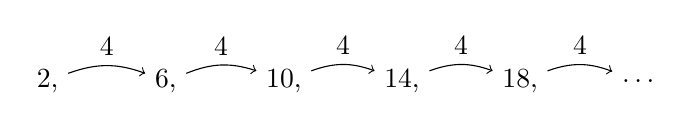
\begin{tikzpicture}[node distance=1.5cm]
    \node (a1) {$2$,};
    \node (a2) [right of=a1] {$6$,};
    \node (a3) [right of=a2] {$10$,};
    \node (a4) [right of=a3] {$14$,};
    \node (a5) [right of=a4] {$18$,};
    \node (a6) [right of=a5] {$\ldots$};

    \path[->] (a1) edge [bend left=20] node[above]{$4$} (a2);
    \path[->] (a2) edge [bend left=20] node[above]{$4$} (a3);
    \path[->] (a3) edge [bend left=20] node[above]{$4$} (a4);
    \path[->] (a4) edge [bend left=20] node[above]{$4$} (a5);
    \path[->] (a5) edge [bend left=20] node[above]{$4$} (a6);
  \end{tikzpicture}
  \end{image}
  
  We can describe this sequence explicitly or recursively. In fact:
  
  This sequence is given explicitly by the function $a_n=\answer[given]{4n - 2}$ for $n \geq 1$.
  
  This sequence is given recursively by the rule $a_1 = \answer[given]{2}$ and $a_{n+1} = a_n +
  \answer[given]{4}$. 

\begin{exercise}
What is $a_{504}$ for this sequence?

\[
a_{504}=\answer{2018}
\]

Which rule is easier to use to find this by hand?

\end{exercise}
  
\end{exercise}
\end{exercise}
\end{document}
